%% LyX 2.1.3 created this file.  For more info, see http://www.lyx.org/.
%% Do not edit unless you really know what you are doing.
\documentclass[english]{article}
\usepackage[latin9]{inputenc}
\usepackage{amsmath}
\usepackage{amssymb}
\usepackage{graphicx}
\usepackage{esint}
\usepackage{babel}
\begin{document}
\section{1}

\section{(a)}

(i) If there is not a $v\in V$ s.t. $Tv=w$ , then this correspond
to case(i)

(ii) If there is at least one $v*\in V$ s.t. $Tv*=w.$ Then we prove
that the solution set is $v*+X$ where $X=\{x|Tx=0\}$ and is a subspace.

First prove that $X$ is a subspace. If $x_{1},x_{2}\in X$, $T(x_{1}+x_{2})=Tx_{1}+Tx_{2}=0+0=0,$
so $x_{1}+x_{2}\in X.$ Also $T(kx_{1})=k(Tx_{1})=k0=0,$$kx\in X.$

So $X$ is a subspace.

Then prove that the solution set $S$ is $v*+X$.

For all $v=v*+x,x\in X$ $Tv=Tv*+Tx=Tv*=w$, so $v*+X\subseteq S$.

Also, $\forall s\in S,T(s-v*)=Ts-Tw*=w-w=0$, so $(s-v*)\in X$ ,
so $S\subseteq v*+X$

So we have proved that $S=v*+X$.

If in case that $X=\{0\}$ , then $v*$ is the only solution, that
corresponds to case (ii)

If $X$ is a subspace of finite dimension , then that corresponds
to case (iii)

(b)

If $T$ is injective and $w$ is in range $T$ , then we have only
solution(case 2).

If $T$ is not injective and $w$ is in range $T$, then we have case
3.(Solution forms a affine space)

If $w$ is not in range $T,$then we have case 1.(No solution)

(c)

As we have shown in (a) , $X$ is the null space of $T$. The dimension
of $X$ is the dimension of $V$ minus the dimension of $TV$.

(d) If $\forall w\in W$ one can find $v\in V$ s.t. $Tv=w.$Then
the range of $T$ which we note as subspace $S$, $W\subseteq S$.
We assmue $V=span\{e_{1},e_{2}...e_{n}\}$

where n is the dimension of $V$. We can prove that $S=span\{Te_{1},Te_{2},Te_{3}...Te_{n}\}$.
This is easy to prove. Since $\forall v\in V,$ assume $v=k_{1}e_{1}+k_{2}e_{2}+...+k_{n}e_{n}$,

$Tv=T(k_{i}e_{i})=k_{i}Te_{i}\in span\{Te_{i}\}$. So $S=span\{Te_{1},Te_{2},..,Te_{n}\}$.
So $dim(S)\leq dim(V)<dim(W)$. So $W\nsubseteq S.$ So there must
be some $w\in W$ not in $S$.

(e)

Since $S\subseteq W$, that means $dim\{span\{Te_{1},Te_{2},...Te_{n}\}\}\leq dim(W)<dim(V)=n$.
That means $\{Te_{i}\}$ cannot be linear independent. So that there
must be a set of non zero coefficients $\{k_{i}\}$ such that $T\Sigma k_{i}e_{i}=0.$
That means the null space of $T$ (noted as $X$)is at least one dimensional.
So if $Tv*=w*$, $v*+X$ is the solution set of $Tv=w*$. So $w*$
has more than 1 solution.

\section{2}

(a) Since all the n order polynomials can be expressed as $p(x)=\Sigma_{i=0}^{n}k_{i}x^{i}$and
all the $\Sigma_{i=0}^{n}k_{i}x^{i}$ belongs to $P_{n}(R)$,so $P_{n}(R)=span\{1,x,x^{2}...x^{n}\}$

Then let's prove that $\{1,x,x^{2},...,x^{n}\}$ are linear independent.
This is been proved in last hw set. 

(b)

Assume $e_{n}=x^{n}$ then $D(e_{n})=nx^{n-1}=n(e_{n-1})$$(n>1)$
and $D(e_{0})=0$ so we can write the operator in matrix form . 

$D_{ij}=j\delta_{i+1,j}(i=0,1,2,..n;j=0,1,2,3,...n+1)$

for example $D=\begin{array}{ccccc}
0 & 1 & 0 & 0 & 0\\
0 & 0 & 2 & 0 & 0\\
0 & 0 & 0 & 3 & 0\\
0 & 0 & 0 & 0 & 4\\
\\
\end{array}$ for $n=4$

(c)

$M(e_{n})=e_{n+1}$, so $M_{ij}=\delta_{i-1,j}(i=0,1,2,3,...n+1;j=0,1,2,3...,n)$

for example $D=\begin{array}{ccccc}
0 & 0 & 0 & 0\\
1 & 0 & 0 & 0\\
0 & 1 & 0 & 0\\
0 & 0 & 1 & 0\\
0 & 0 & 0 & 1
\end{array}$ for $n=4$

(d)$(DM)_{ij}=D_{ik}M_{kj}=k\delta_{i+1,k}\delta_{k-1,j}=(i+1)\delta_{i,j}(i,j=0,1,2,3,...n)$

$(MD)_{ij}=M_{ik}D_{kj}=\delta_{i-1,k}j\delta_{k+1,j}=j\delta_{i,j}(i,j=0,1,2,3...n+1)$

(e)orignally the $MD$ operator is from $P_{n+1}(R)$ to $P_{n+1}(R)$,
if we restrict it to $P_{n}(R)$, then we eliminate the $n+1$ row
and $n+1$ column of the matrix.

$R_{ij}=j\delta_{i,j}(i,j=0,1,2,3...n)$

(f) $DM-R$ can be seen as the commute of operator $D$ and $M$

$(DM-R)_{i,j}=(i+1)\delta_{i,j}-j\delta_{i,j}=\delta_{i,j}$ that
is the identity operator.

\section{3}

(a)All the functions that are Riemann intergrable and the the Riemann
integral of the function is also Riemann integrable is in the range
of the linear map $D^{2}.$

For example, the dirichlet function is not in the range.

$D^{2}f(x)=0$, then it is easy to solve this ode and get $f(x)=a+bx$.
So the kernel of $D^{2}$operator are all the first and zero order
polynomials. It is a $2$ dimensional space $span\{1,x\}$

(b)We can solve the ODE by integral. 

$u"(x)=f(x)$ $u'(x)=C_{1}+\int_{0}^{x}f(x')dx'$$u(x)=C_{2}+\int_{0}^{x}(C_{1}+\int_{0}^{u}f(x')dx')du=C_{2}+C_{1}x+\int_{0}^{x}\int_{0}^{u}f(x')dx'du$
So the ODE donot have a unique solution. The solution to this ODE
is a special solution plus a linear space that is the kernel of the
$D^{2}$ operator.

(c)Let's node $F(x):=\int_{0}^{x}\int_{0}^{u}f(x')dx'du.$ If we have
two boundary conditions, then we need to enforce 

$u(0)=F(0)+C_{2}=a$ and $u(1)=F(1)+C_{1}+C_{2}=b$

Since $F(0)=0,$$C_{2}=a$ and $C_{1}=b-a-F(1)$

So we have a unique solution.

(d) Yes. It has a unique solution. Since in (2) we have n+1 linear
relations and $n+1$ unknowns ($x_{0},x_{1}...x_{n}$). And we can
show later that the $n+1$ relations are linearly independent.

(e)

A=$\begin{bmatrix}\\
\\
\\
\begin{array}{cccccccc}
-1 & 2 & -1\\
 & -1 & 2 & -1\\
 &  & -1 & 2 & -1\\
 &  &  & ... & ... & ...\\
 &  &  &  & -1 & 2 & -1\\
 &  &  &  &  & -1 & 2 & -1\\
1\\
 &  &  &  &  &  &  & 1
\end{array}\\
\\
\\
\\
\\
\end{bmatrix}$,x=$\begin{bmatrix}\\
\\
\\
\begin{array}{c}
v(x_{0})\\
v(x_{1})\\
v(x_{2})\\
...\\
...\\
...\\
...\\
v(x_{n})
\end{array}\\
\\
\\
\\
\\
\end{bmatrix}$,b=$\begin{bmatrix}\\
\\
\\
\begin{array}{c}
h^{2}f(x_{1})\\
h^{2}f(x_{2})\\
...\\
...\\
...\\
h^{2}f(x_{n-1})\\
a\\
b
\end{array}\\
\\
\\
\\
\\
\end{bmatrix}$

(f)

function{[}results{]} = solver(N,func\_handle,a,b)

A = zeros(N+1);

r = zeros(1,N+1); 

for ii = 1:1:N-1 

A(ii,ii) = -1; 

A(ii,ii+1) = 2; 

A(ii,ii+2) = -1; 

end 

A(N,1) = 1; 

A(N + 1 , N + 1) = 1; 

X = linspace(0,1,N+1); 

h = 1/N; 

for ii = 1:1:N-1 

r(ii) = h\textasciicircum{}2{*}func\_handle(X(ii + 1)); 

end 

r(N) = a; r(N+1) = b;

results = A\textbackslash{}r';

plot(X,results); 

end 

solution = solver(10,@f,0,1); 

hold on 

solution = solver(100,@f,0,1); 

hold on 

solution = solver(1000,@f,0,1); 

(g)

The exact solution to (1) is :

$F(x)+C_{1}x+C_{2}$

$F(x)=\int_{0}^{1}\int_{0}^{x'}(-4\pi^{2})sin(2\pi u)dudx'=sin(2\pi x)$

$C_{2}=a=0$

$C_{1}=b-a-F(1)=1-0-0=1$

So the solution is $sin(2\pi x)+x$

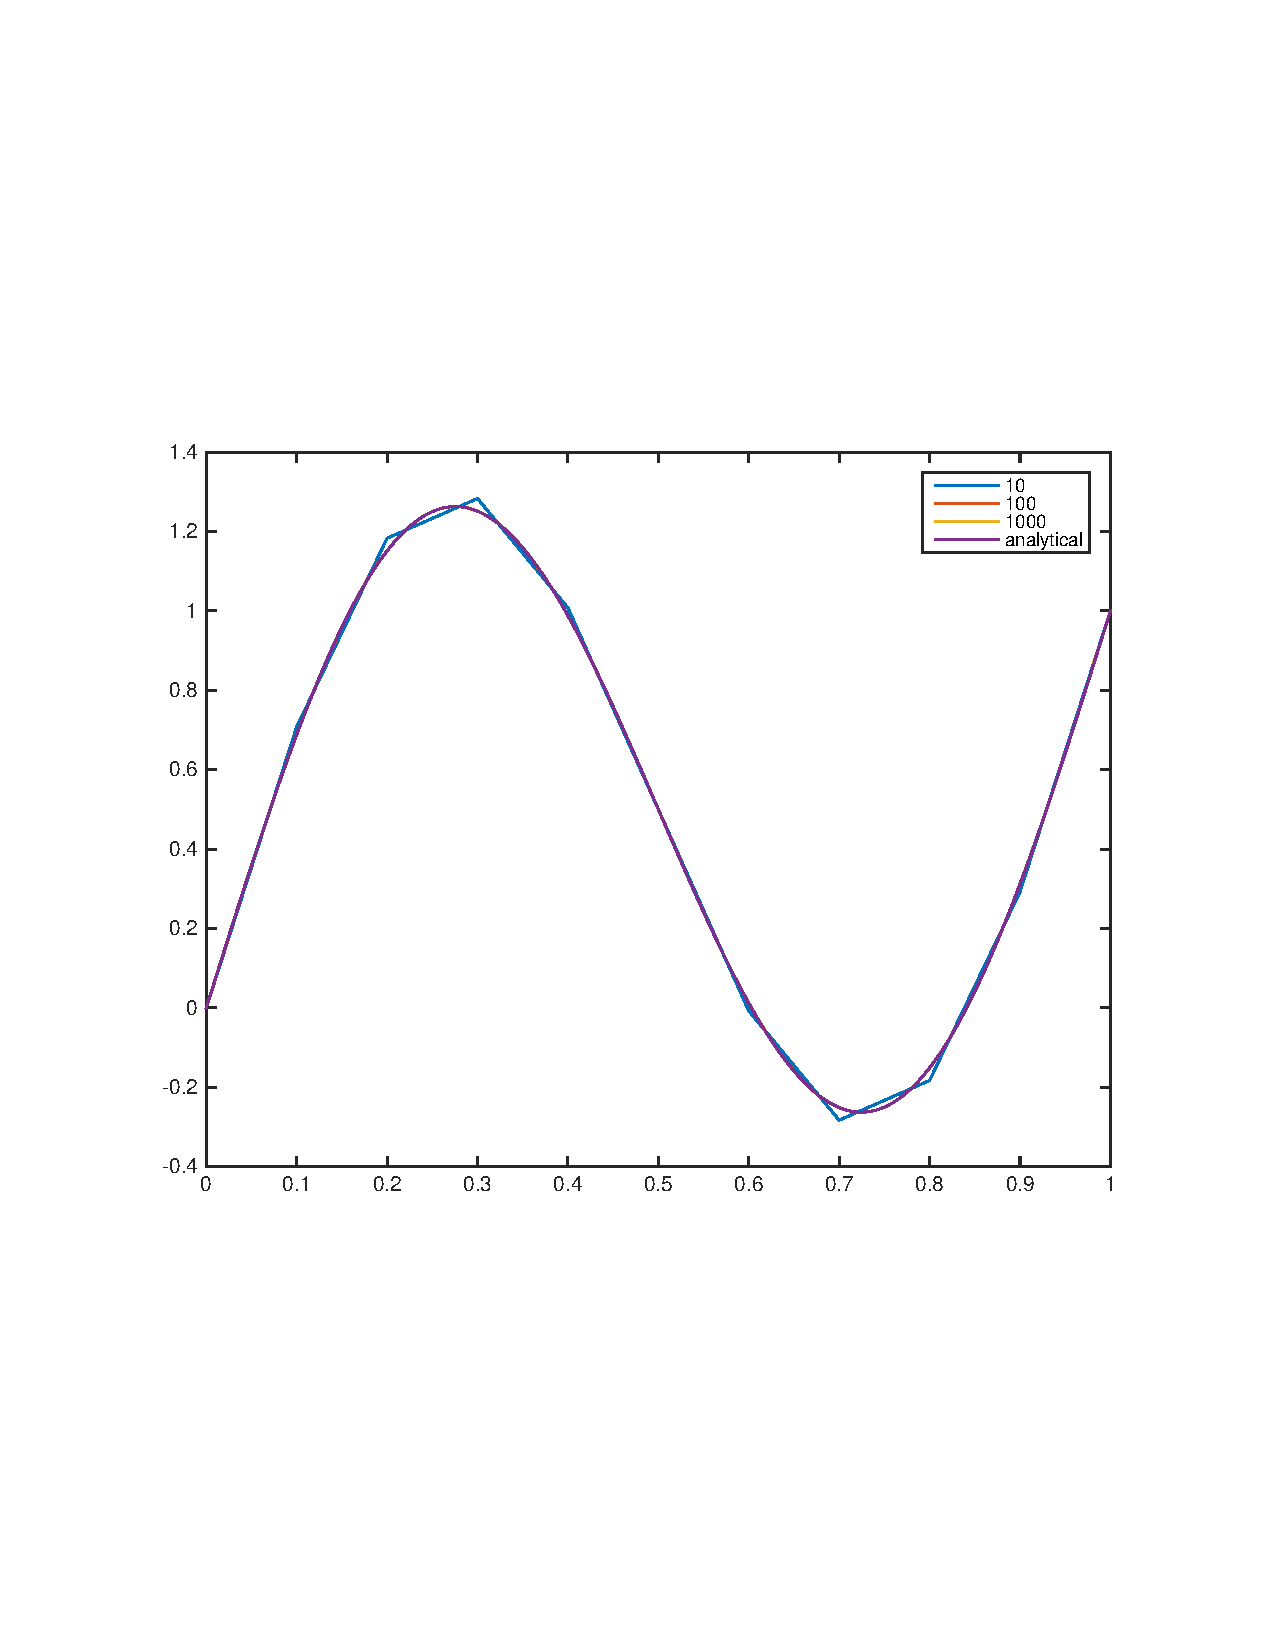
\includegraphics{101001000}

(h)

The problem (1) has a solution since $cos(e^{3x})$ is Rieman integrable
for twice.

The problem(2) also has a solution. And that should converge to the
analytical solution in (1)

Here shows the plot.

We cannot write the integral in a simple analytical form .

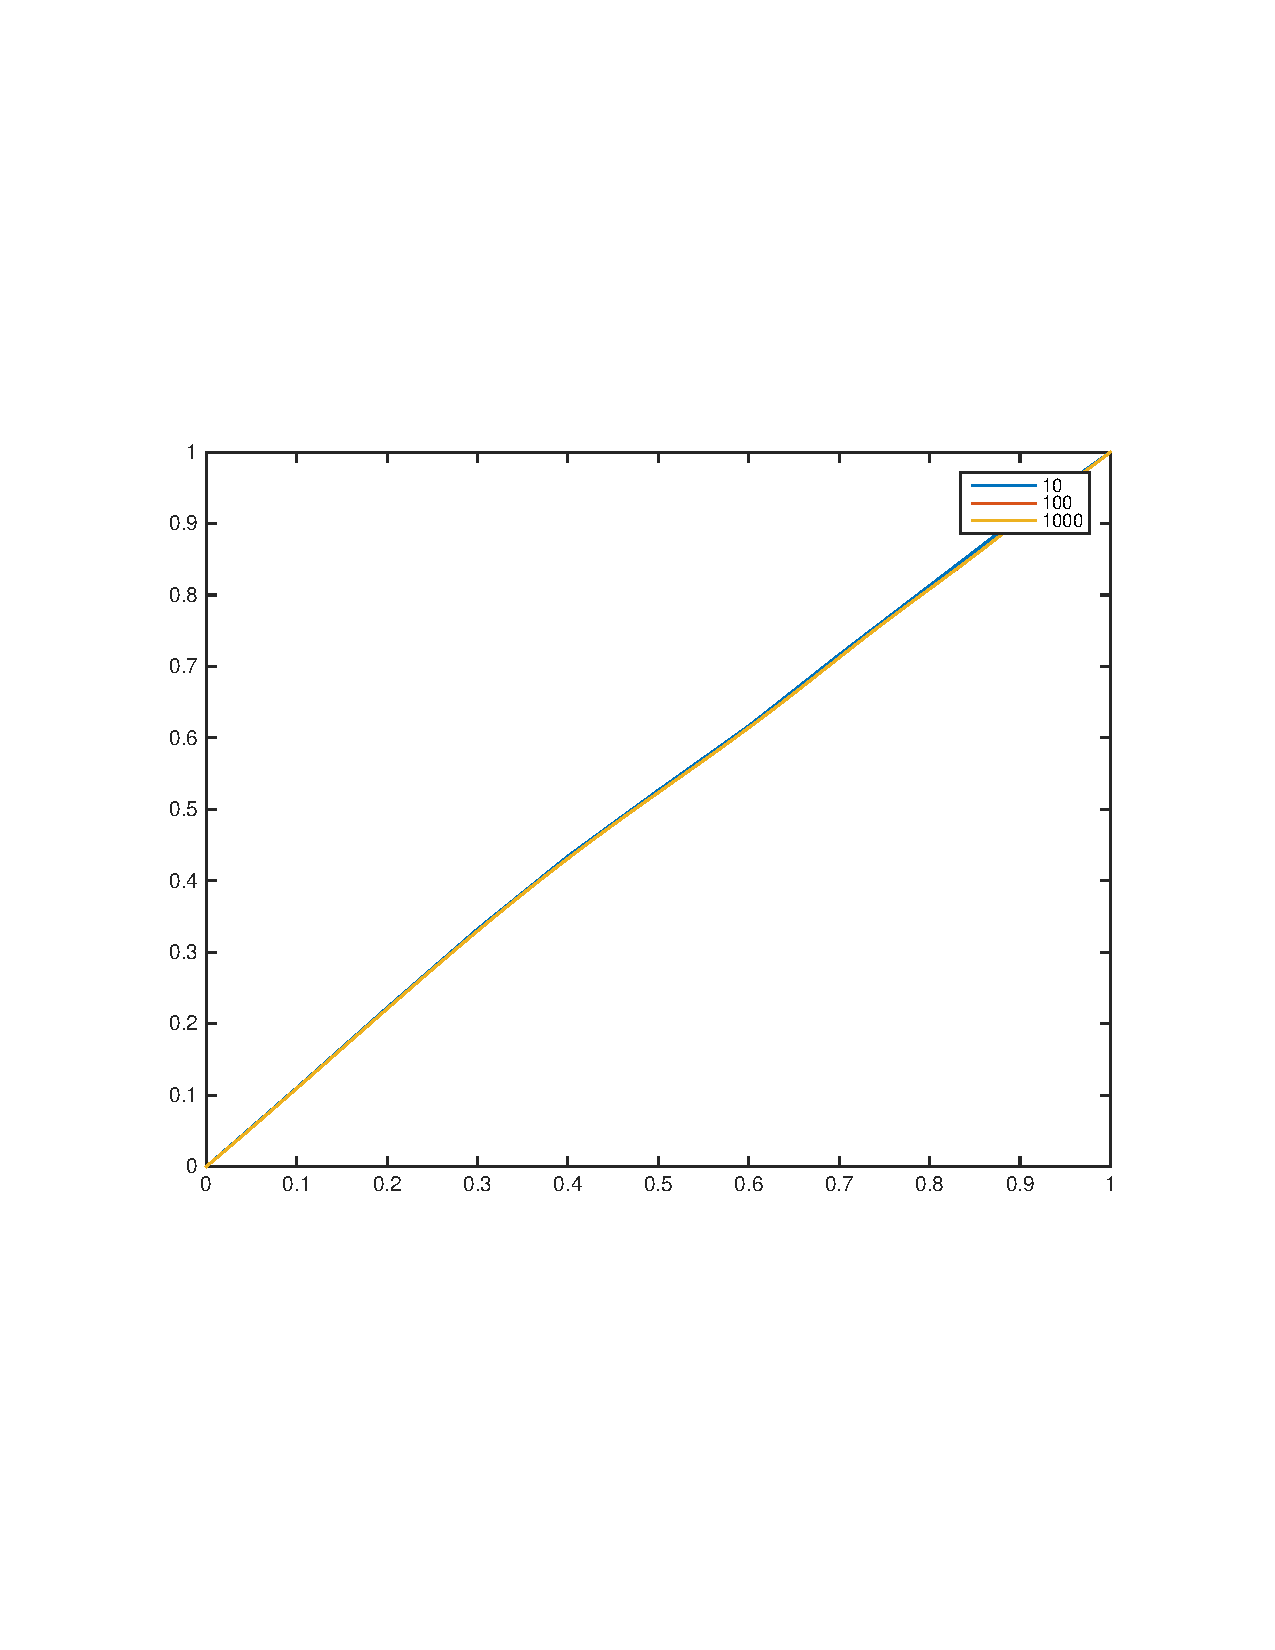
\includegraphics{unknownfunc}
\end{document}
